\documentclass[12pt]{article}
\usepackage{authblk}
\usepackage{graphicx}
\usepackage{multirow}
\usepackage{tikz}
\usepackage{caption}
\usepackage{subcaption}
\usepackage{comment}
\usepackage{float}
\usetikzlibrary{positioning}
\usepackage[utf8]{inputenc}
\setlength{\arrayrulewidth}{.5mm}
\setlength{\tabcolsep}{12pt}
\renewcommand{\arraystretch}{.5}
\usepackage[export]{adjustbox}
\graphicspath{{C:/Users/Gauri/Pictures}}
\title{\textbf{Evaluation of vector libraries on AJIT}}
\author[1]{Gauri Patrikar }

\begin{document}

\maketitle
\begin{abstract}

Vector or SIMD (single instructions multiple data) instructions are a class of instructions that enable parallel processing. It performs the same operation on multiple input data streams at the same time, exploiting data level parallelism, hence enhancing the performance.
AJIT processor is an implementation of the SPARC-V8 ISA. 
We have added 64 bit vector instructions to the existing 32 bit SPARC V8 ISA, implemented on the AJIT 64 bit processor. These instructions use 2 32 bit registers to execute a 64 bit instruction.

We developed String and blas libraries using the SPARC V8 assembly with the newly added extensions to the AJIT processor. DSP functions using these blas libraries were also implemented. 
 
The performance for implemented string and blas functions is characterized and improvement in performance of upto 92\% for string and upto 96\% for blas was observed.The performance is measured in terms of clock cycles required.

 \end{abstract}

\section{Introduction}
Vector instructions are widely used in AI, DSP and graphics applications to significantly enhance the performance of these operations. They perform operations on multiple data sets in a single clock cycle. 
The SPARC V8 is a 32 bit ISA, which has no vector instructions. For the AJIT 64 bit processor, we have extended the ISA to include 64 bit instructions, some of which are vector instructions. Using these instructions, we have developed string and linear algebra libraries. These libraries have shown significant improvement over original functions which use the 32 bit SPARC ISA. 
These newly developed libraries an be used for various appplications in AI/DSP etc. A couple of DSP functions are also developed to demonstrate the enhanced performance.

The paper is divided into following sections - section 3 details the vector instructions, section 4 talks about the SPARC ABI, section 5 gives specifications of all implemented libraries, section 6 gives the testing methodology, section 7 outlines the results, and section 8 concludes the paper.

\section{AJIT Vector Instructions}

The AJIT processor is based on the 32 bit SPARC V8 ISA. New assembly instructions that perform 64 bit operations have been added to enhance the performance.
They can be categorized as follows - 
\begin{itemize}
    \item Integer unit extensions - 64 bit arithmetic-logic-shift instructions. These accept 64 bit input operands and the output is also 64 bits.
    \item SIMD - These instructions are vector instructions which work on two source registers (each a 64 bit register pair), and produce a 64-bit vector result.  The vector elements can be 8-bit/16-bit/32-bit.
    \item SIMD (bytereduce) - These instructions are vector instructions which reduce a 64 bit source register to a destination using an associative operation.    
    \item Floating point vector -  These are vector float operations which work on two single precision operand pairs to produce two single precision results.
    \item  Half precision conversion instructions - These instructions allow conversion between IEEE half-precision
    numbers and IEEE single/double precision numbers and integers.      
\end{itemize}

These instructions are performed in a single clock cycle and  help reduce number of operations, hence making a program much faster.\newline

Strings terminate with a null byte. Hence, finding the zeroth byte is important. Using the zbytedpos (a type of byte reduce instruction, gives the positions of zero bytes in a 64 bit input) instruction, we can find the null byte in a 64 bit number in one instruction itself. 
In case of other instructions also, operations are performed two at once, for eg., multiplying up to 8 8 byte inputs at once. 


\section{SPARC ABI}

SPARC ABI is a calling convention used when an assembly program needs to be called using a C program.  It gives the protocol for argument passing, writing the prologue and epilogue of the assembly functions and so on. This ensures that the process of shifting between the C and the assembly programs is seamless. 

The libraries have been written in assembly, simply because generating a compiler was a more complex task.
These libraries can be called from a C program, and hence the SPARC ABI protocol is used.

\section{Implemented functions}
We have implemented 5 string functions and 5 blas functions. The blas functions have been written for 4 data types. 2 DSP functions using the blas libraries were also written.
Th list of libraries is given blow, followed with restrictions and usage of these libraries.


\subsection{String}
The following functions are being implemented here (all functions input two strings) - 
\begin{enumerate}
    \item strcpy - copies source string to destination 
    \item strncpy - copies n bytes of source string to destination.
    \item strcmp  - compares two input strings
    \item strcasecmp - compare two input strings ignoring case of the character
    \item strcat  - concatenates source string at the end of destination string.
\end{enumerate}

\subsection{Blas}
  
Each of the given functions are implemented for 5 data types - 8, 16 and 32 bit unsigned int and single precision floating point.
\begin{enumerate}
    \item asum - sum of absolute values of an array
    \item scal - scales elements of array by a constant
    \item axpy - implements  on each element of the array
    \item dot -  computes the dot product between two arrays
    \item Isamax - finds the largest element of the array
\end{enumerate}\



Using these Blas libraries following functions were implemented - 
\begin{enumerate}
    \item FFT
    \item Convolution
\end{enumerate}

\subsection{Restrictions}

As we were dealing with 64 bit operations, aligning the inputs to 64 bit boundaries was required. It is the users responsibility to make sure all inputs are aligned to make use of the 64 bit libraries.

\subsection{Usage}

All of the mentioned functions can be called from a C program. 

\section{Testing framework}


We have used a cross-compiler to generate SPARC-V8 executable code.
We have added  the 64 bit extensions to the binary utils, hence the 64 bit instructions can be assembled.

The libraries have been tested on the AJIT processor core on an FPGA prototyping board (KC705).

We have compared the string libraries with the existing uclibc C string functions. The blas functions are compared to those in the gnu scientific library. The DSP functions were compared by writing both in C and adding inline assembly for the vector case.

\section{Results}
The results are given in terms of clock cycles required by each function.  

\subsection{String}

For string libraries, functions are compared at various string lengths. taken in multiples of 160 bytes. We have tested for 160*K+n, where k = 1,2,4,8 and n = 0 to 7. In each case improvement is noted.

\begin{figure}[H]
     \centering
     \begin{subfigure}[b]{0.4\textwidth}
         \centering
         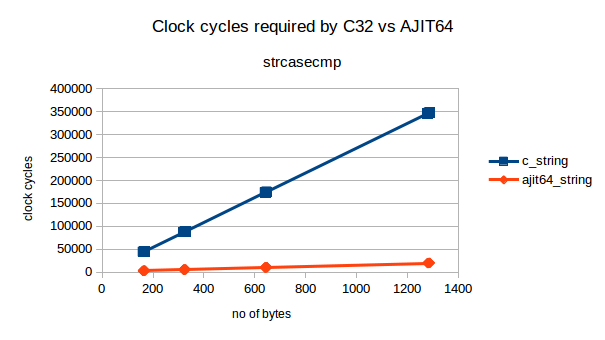
\includegraphics[width=\textwidth]{strcasecmp.png}
         \caption{strcasecmp}
     \end{subfigure}
     \hfill
     \begin{subfigure}[b]{0.4\textwidth}
         \centering
         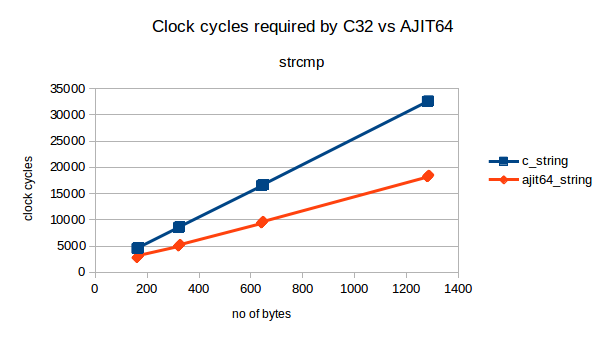
\includegraphics[width=\textwidth]{strcmp.png}
         \caption{strcmp}
         \end{subfigure}
     \hfill
     \begin{subfigure}[b]{0.4\textwidth}
         \centering
         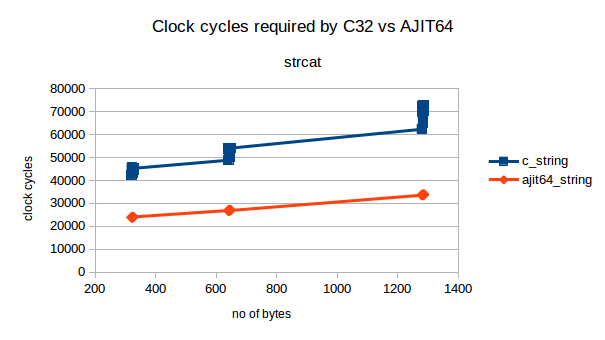
\includegraphics[width=\textwidth]{strcat.png}
         \caption{strcat}
     \end{subfigure}
       \hfill
     \begin{subfigure}[b]{0.4\textwidth}
         \centering
         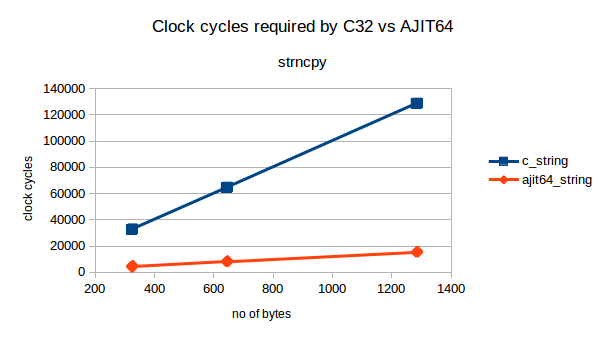
\includegraphics[width=\textwidth]{strncpy.png}
         \caption{strncpy}
         \end{subfigure}
       \hfill
     \begin{subfigure}[b]{0.4\textwidth}
         \centering
         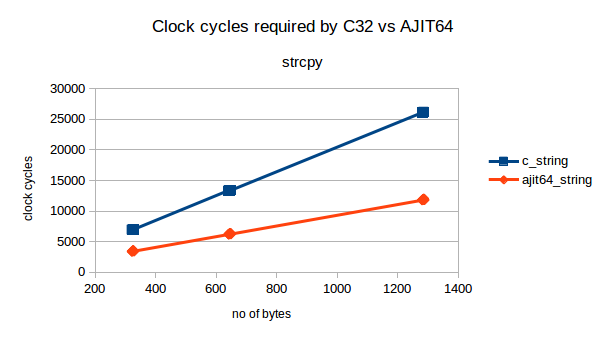
\includegraphics[width=\textwidth]{strcpy.png}
         \caption{strcpy}
     \end{subfigure}
        \caption{String functions}
        \label{fig:three graphs}
\end{figure}


\subsection{Blas}

For blas libraries, lengths of have been taken from 200 to 3200 in increments of 600. For each function comparison of one data type out of the four is given.

\begin{figure}[H]
     \centering
     \begin{subfigure}[b]{0.4\textwidth}
         \centering
         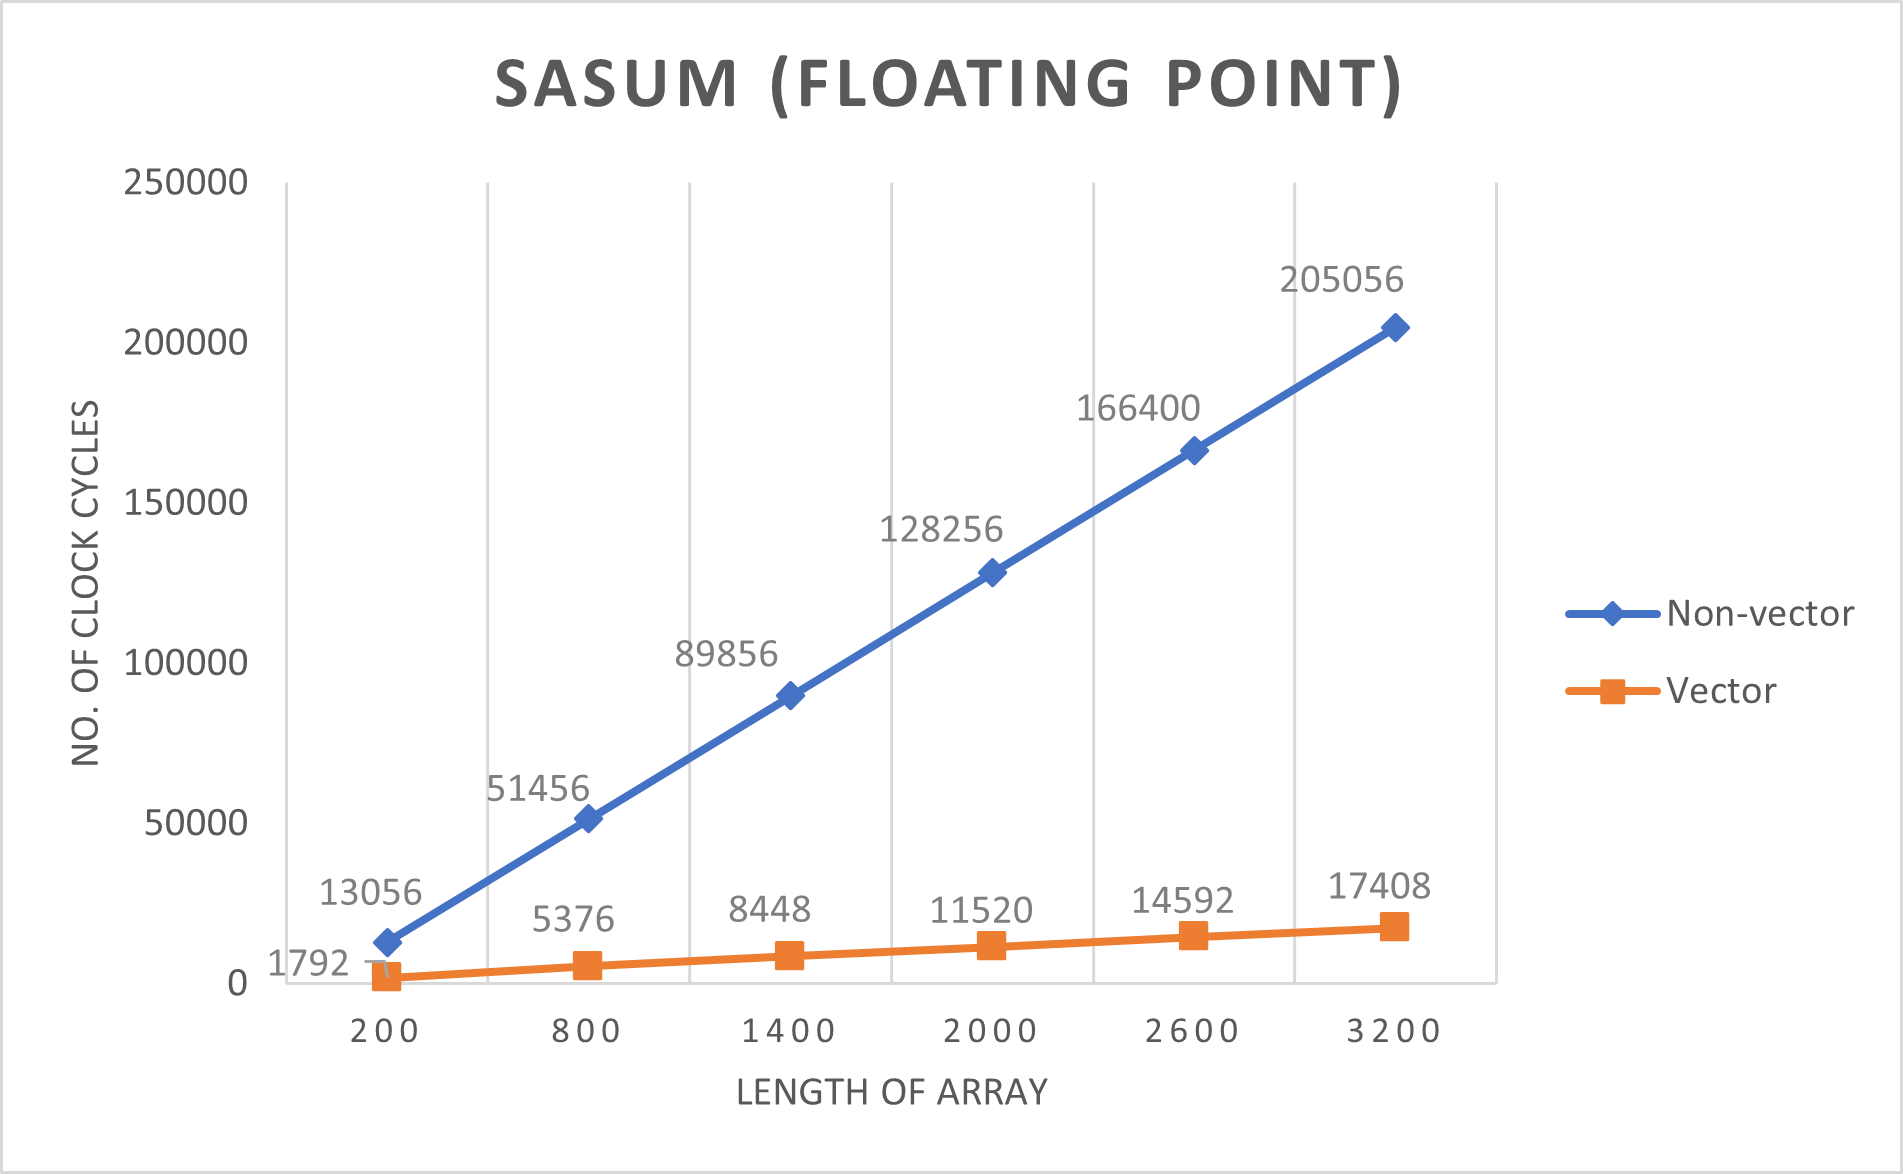
\includegraphics[width=\textwidth]{sasum_floating.png}
         \caption{sum}
     \end{subfigure}
     \hfill
     \begin{subfigure}[b]{0.4\textwidth}
         \centering
         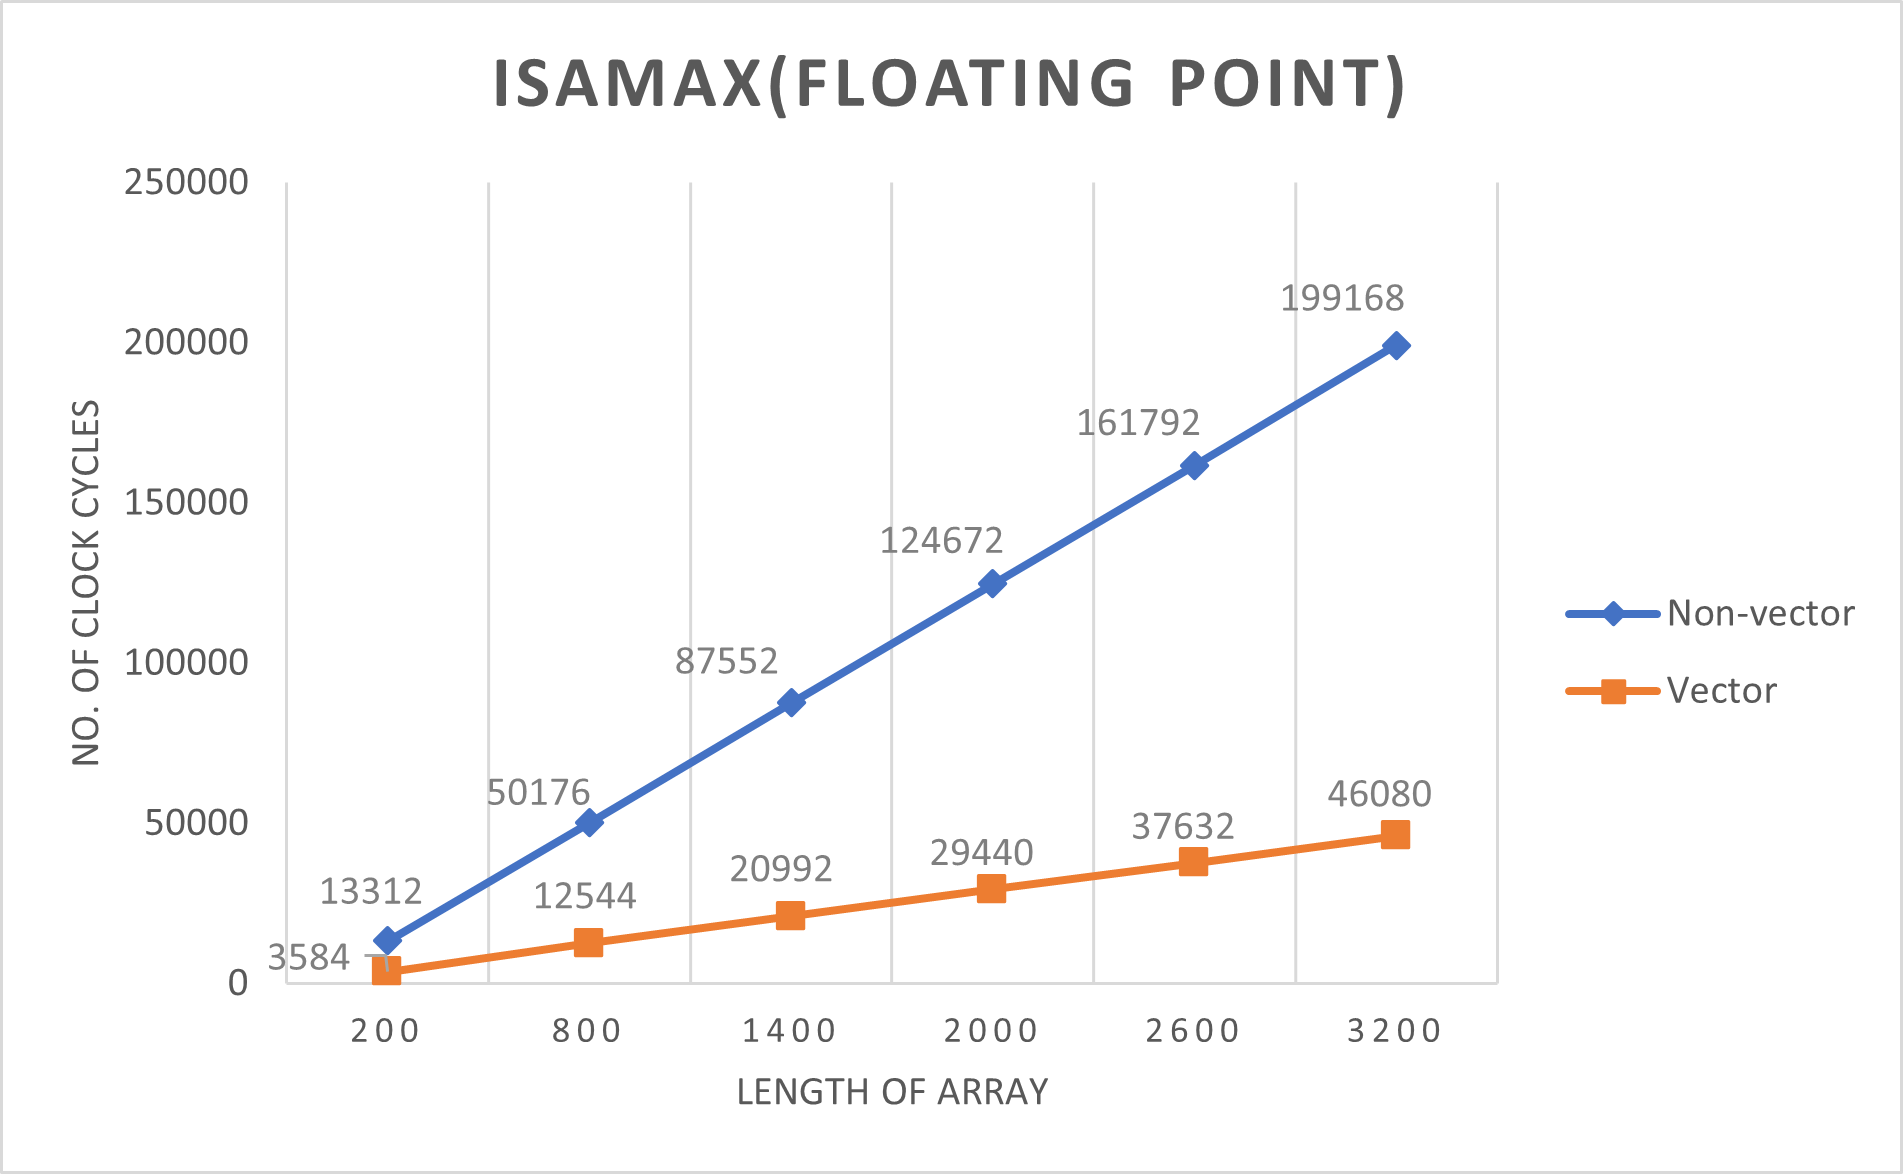
\includegraphics[width=\textwidth]{isamax.png}
         \caption{max}
         \end{subfigure}
     \hfill
     \begin{subfigure}[b]{0.4\textwidth}
         \centering
         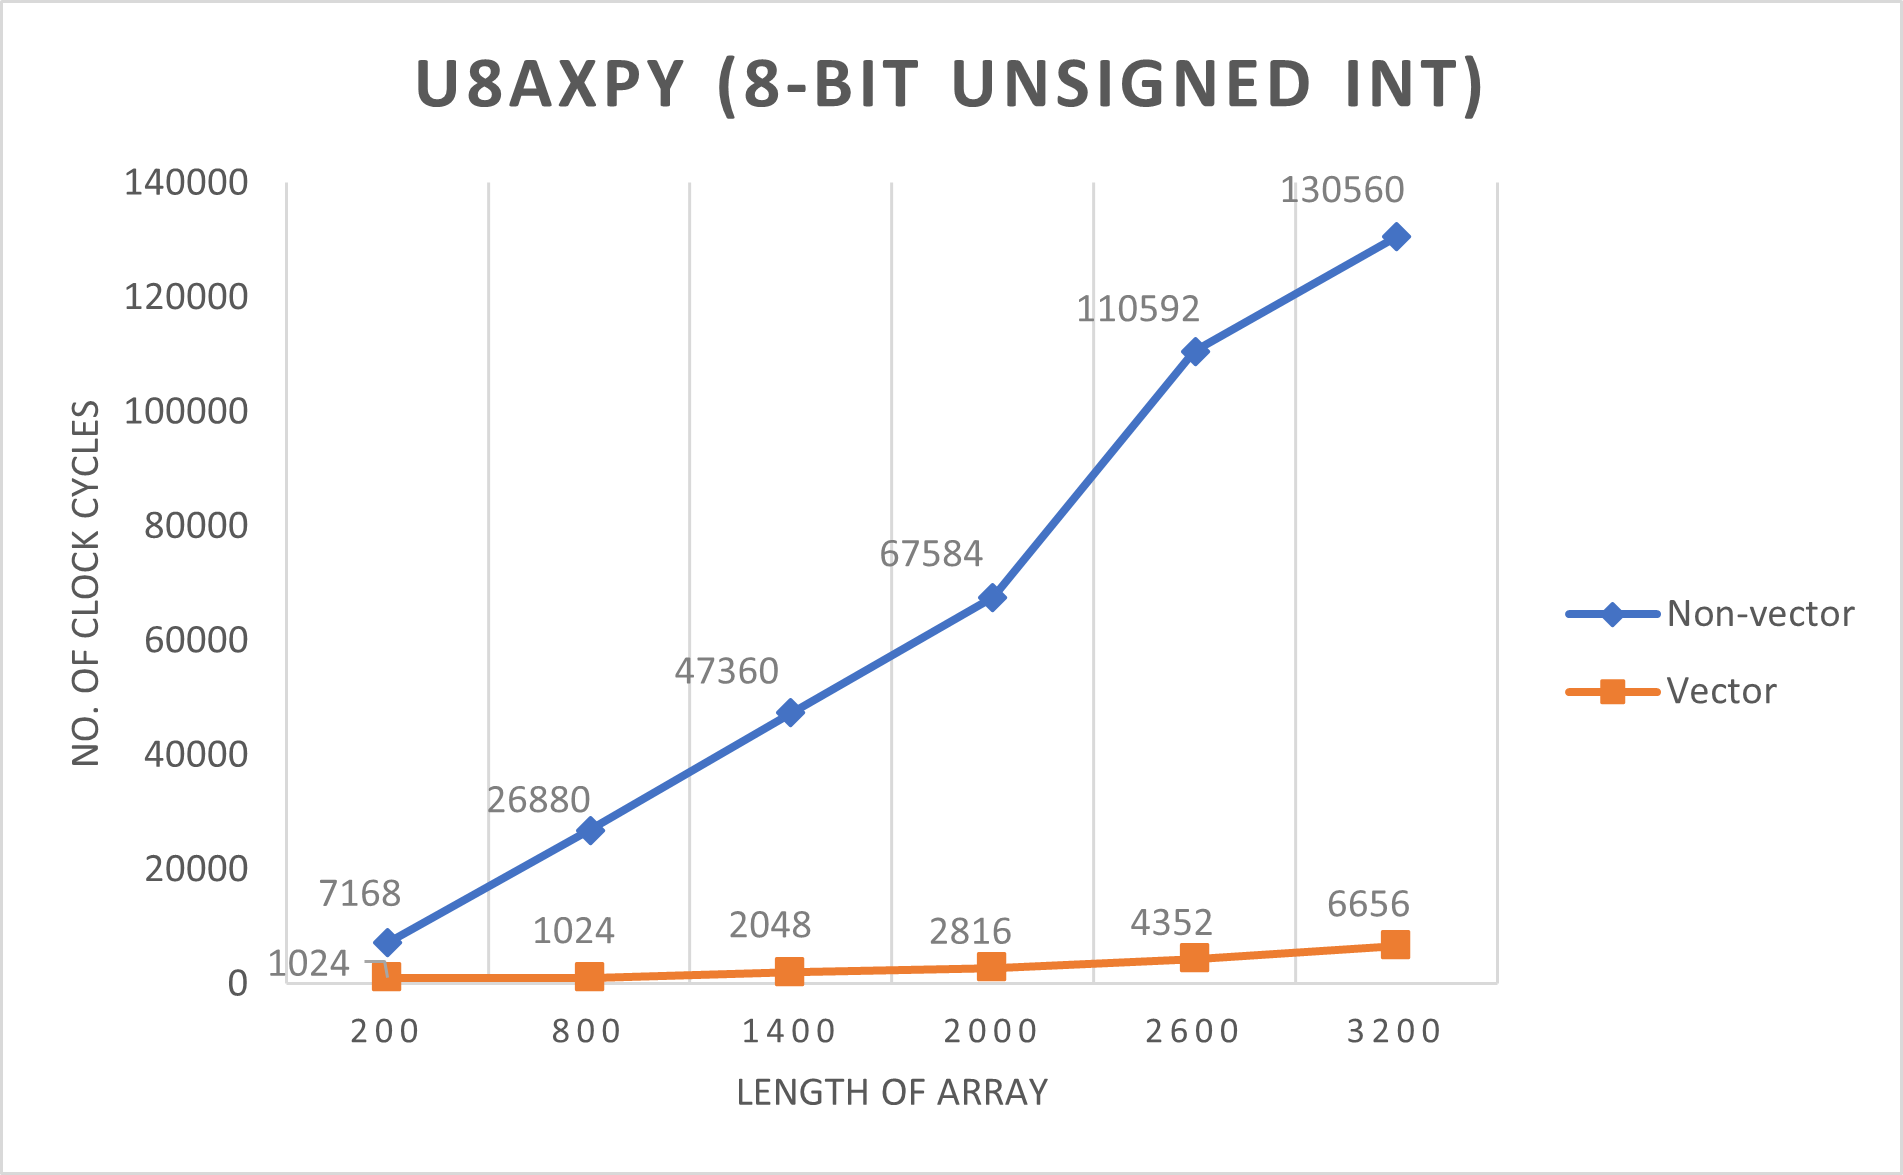
\includegraphics[width=\textwidth]{u8axpy.png}
         \caption{u8axpy}
     \end{subfigure}
       \hfill
     \begin{subfigure}[b]{0.4\textwidth}
         \centering
         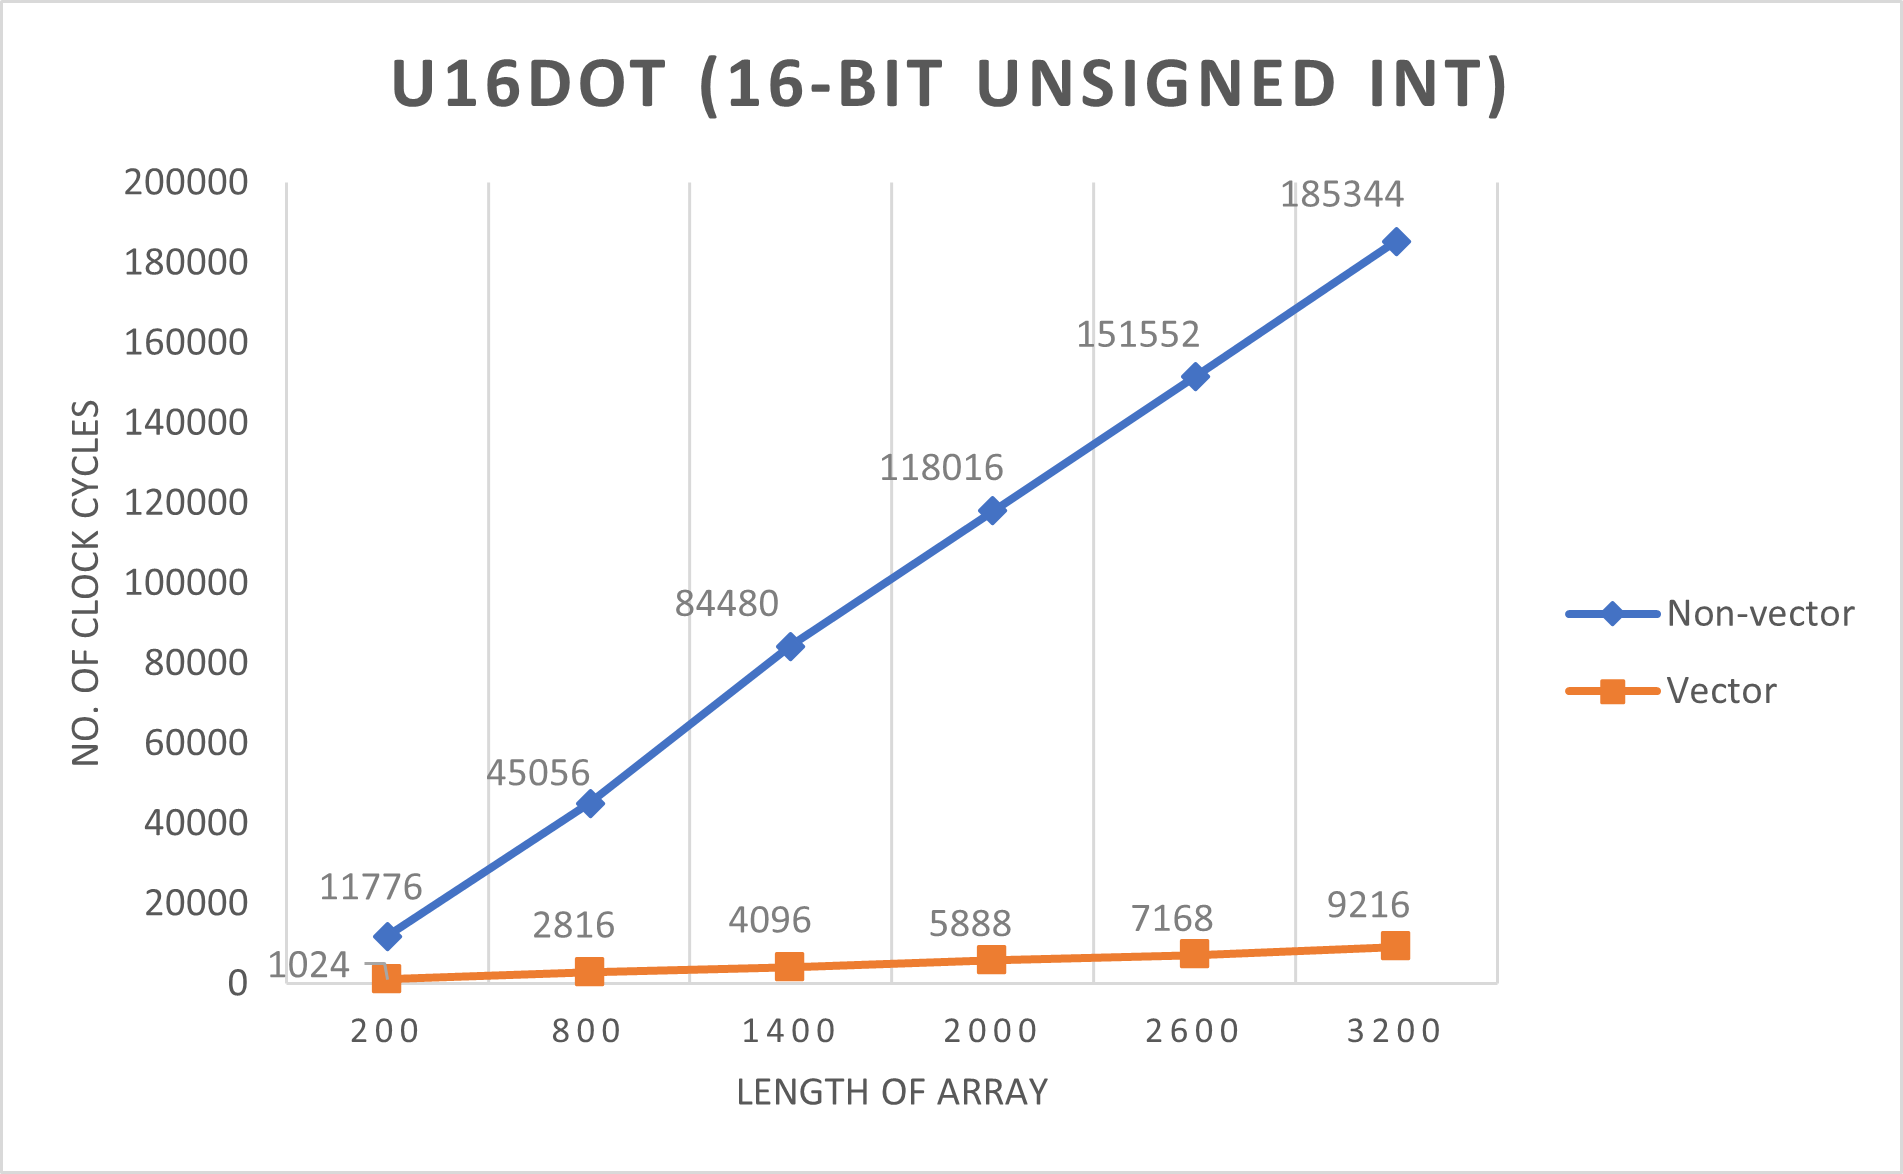
\includegraphics[width=\textwidth]{u16dot.png}
         \caption{dot product}
         \end{subfigure}
       \hfill
     \begin{subfigure}[b]{0.4\textwidth}
         \centering
         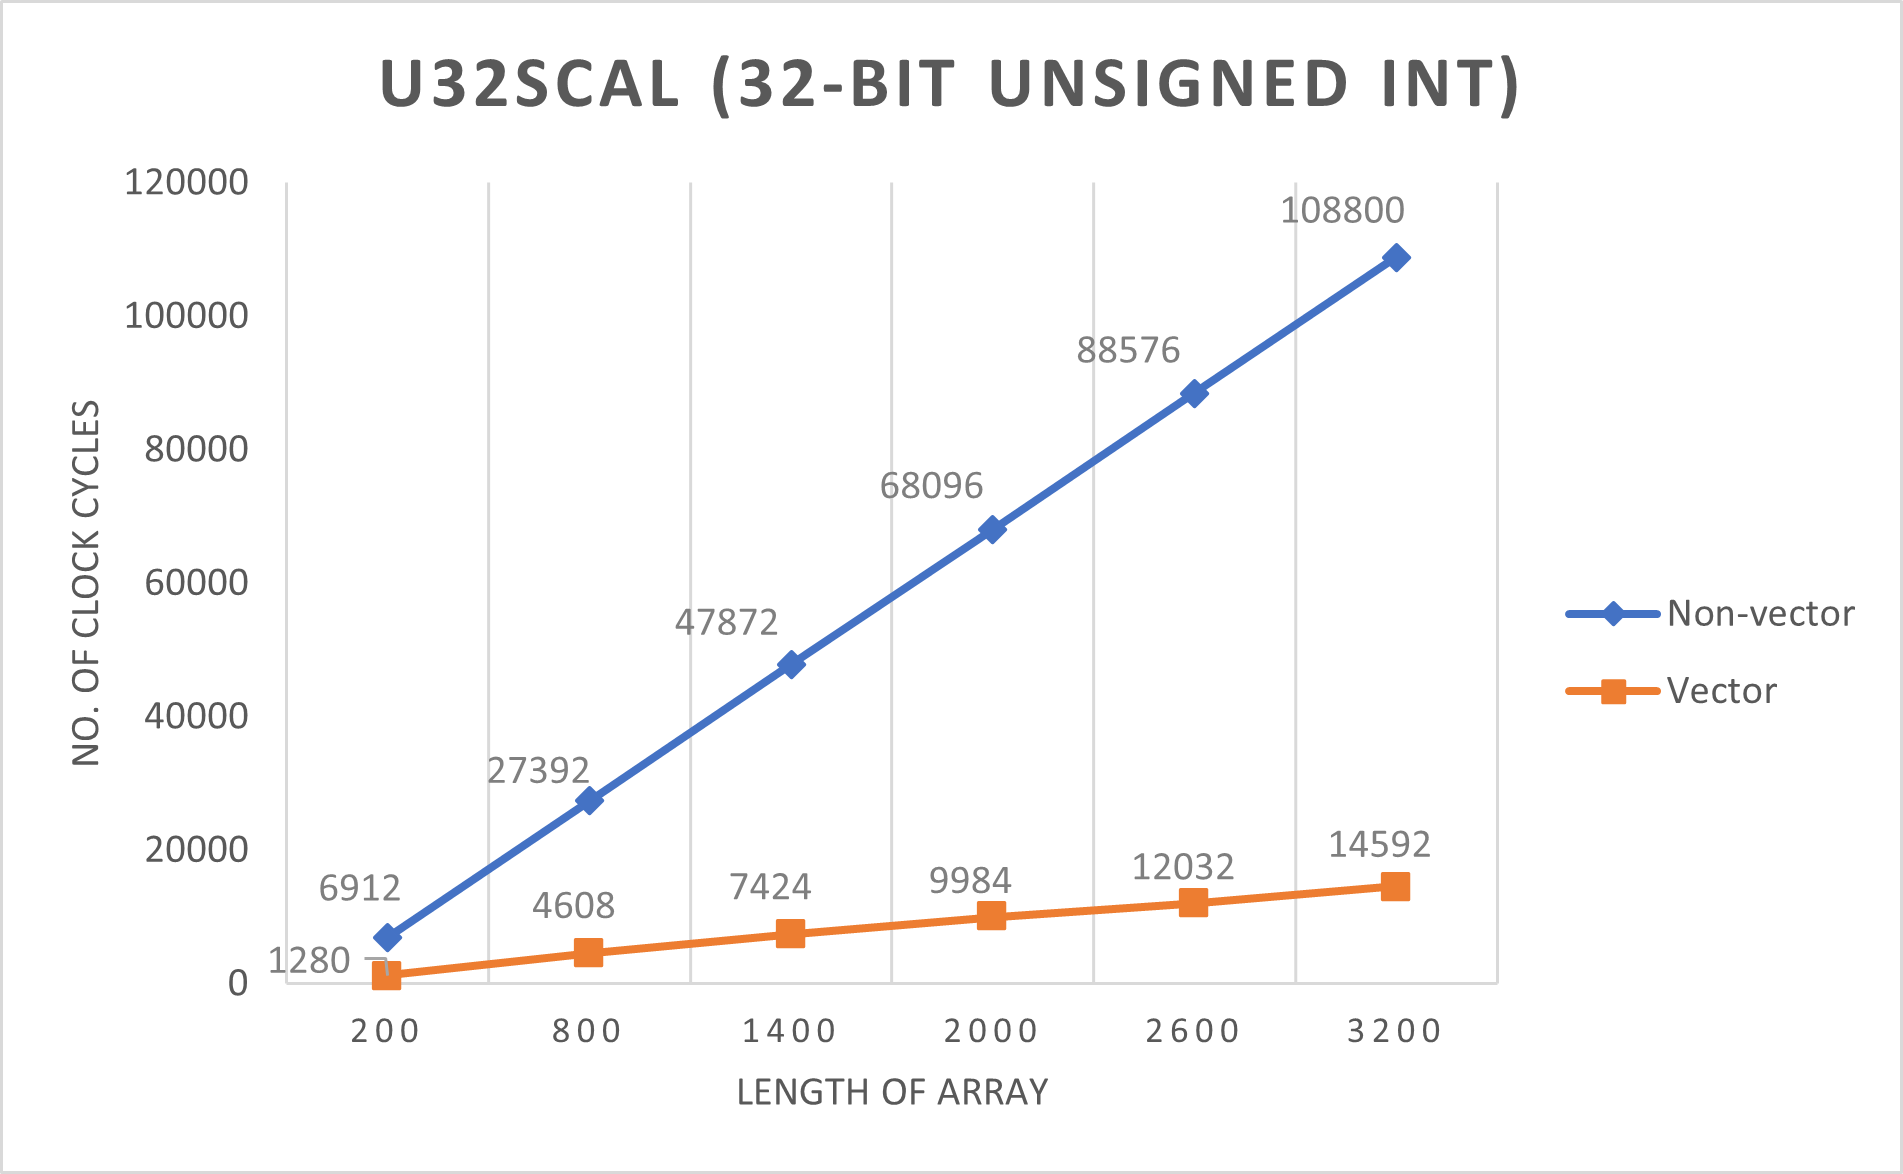
\includegraphics[width=\textwidth]{u32scal.png}
         \caption{scaling}
     \end{subfigure}
        \caption{Blas functions}
        \label{fig:three graphs}
\end{figure}



\section{Conclusions}
In this paper we have presented newly developed vector string and blas libraries. All of libraries have shown significant improvement of up to 96\% compared to their non vectored equivalent. DSP applications making use of these libraries also showed improvement of . All these functions have multiple iterations as the main function. These iterations are reduced greatly due to the use of 64 bit and vector instructions, which provides the performance enhancement. 



























\end{document}
